\documentclass[12pt]{book}
\usepackage[top=1in, bottom=1in, left=1in, right=1in]{geometry}
\usepackage[onehalfspacing]{setspace}
\usepackage[french]{babel}
              
\usepackage{amsmath, amssymb, amsthm}
\usepackage{mathrsfs}
\usepackage{amsfonts}
\usepackage{mathtools}
\usepackage{stmaryrd}

\newcommand{\defeq}{\vcentcolon=}
\newcommand{\eqdef}{=\vcentcolon}
                   
\usepackage{enumerate, enumitem}
\usepackage{fancyhdr, graphicx, proof, comment, multicol}
\usepackage[none]{hyphenat}
\usepackage{dirtytalk}
\usepackage{proof}
           
\usepackage{graphicx}
\usepackage{tikz-cd}

\usepackage{import}
\usepackage{xifthen}
\usepackage{pdfpages}
\usepackage{transparent}
\newcommand{\incfig}[1]{%
    \def\svgwidth{\columnwidth}
    \import{./figures/}{#1.pdf_tex} 
}
            
\newtheorem{lemma}{Lemme}[section]
\newtheorem{theorem}[lemma]{Théorème}
\newtheorem{cor}[lemma]{Corollaire}
\newtheorem{prop}[lemma]{Proposition}
                    
\theoremstyle{definition}
\newtheorem{definition}[lemma]{Définition}
\newtheorem{example}[lemma]{Exemple}
\newenvironment{comments}{}{}

\theoremstyle{remark}
\newtheorem*{remark}{Remarque}

\newcommand*\quot[2]{{^{\textstyle #1}\big/_{\textstyle #2}}}

\begin{document}
	\chapter{La topologie quotient}
	Dans tout ce chapitre X dénote un espace \emph{topologique}, q une surjection. Sauf mention du contraire lorsqu'il est question d'espaces topologiques une application est considérée continue.

	\section{Théorie générale}
	\begin{definition}[Topologie quotient]
		La topologie quotient sur Y a pour ouverts les sous ensembles $U \subset Y$ tels que $q^{-1}(U)$ est ouvert dans X.
	\end{definition}
	\begin{remark}
		Une caractérisation équivalente de cette topologie peut se faire en définissant les fermés de Y par les fermés de X.
	\end{remark}
	\begin{definition}[Quotient]
		On dit que $q : X \longmapsto Y$ est un quotient si elle est surjective continue et que la topologie quotient induite par q coïncide avec la topologie de Y.	
	\end{definition}
	\begin{prop}
		Si $q : X \longmapsto Y$ est une application surjective continue et ouverte alors q est un quotient et Y est muni de la topologie quotient définie par q.
	\end{prop}
	\begin{proof}
		Si U est ouvert dans Y alors $q^{-1}(U)$ est ouvert dans X par continuité de q. Réciproquement si  $ U \subset Y$ et $q^{-1}(U)$ est ouvert dans X alors par surjectivité de q  \[
			q(q^{-1}(U)) = U
		\] et on en conclut que U est ouvert dans X puisque q est ouverte. 
	\end{proof}
	\begin{remark}
		Ce critère reste valable si q est une application fermée, la preuve est identique en remplaçant les ouverts par des fermés.
	\end{remark}
	\begin{example}
		Il est cependant important de noter que ce critère bien que suffisant n'est \emph{pas} nécessaire. Définissons l'application\\

		\noindent \begin{minipage}{0.5\textwidth}
		\begin{align*}
			q : [0,3] &\longmapsto [0,2]\\
			t &\longmapsto \begin{cases}
				t \text{\; si \;} t \le 1\\
				1 \text{\; si \;} 1 \le t \le 2\\
				t-1 \text{\; sinon}
			\end{cases}
		.\end{align*}
		\end{minipage}
		\hfill
		\noindent \begin{minipage}{0.5\textwidth}
			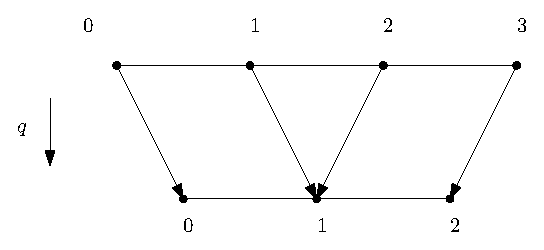
\includegraphics[width=\linewidth]{example_1.eps}
		\end{minipage}\\

		q est une application continue, c'est un quotient pour la topologie euclidienne sur $[0,3], [0,2]$ mais elle n'est pas ouverte,  $(1,2)$ est envoyé sur ${1}$.
	\end{example}

	\begin{prop}
		La composition de deux quotients est également un quotient.
	\end{prop}
	\begin{prop}[Propriété universelle]
		La topologie quotient est la plus fine telle que l'application q soit continue. De plus, $g : Y \longmapsto Z$ est un e application continue si et seulement si	$g \circ q : X \longmapsto Z$ est continue.
	\end{prop}
	\begin{proof}
		Soit U un ouvert d'une topologie sur Y telle que q soit continue. Par continuité de q $q^{-1}(U)$ est ouvert dans X et donc U est ouvert dans Y pour la topologie quotient. 
		Si g est continue $g \circ q$ est continue en tant que composition d'applications continues. Réciproquement, si  $g \circ q$ est continue prenons $V \subset Z$ un ouvert, $(g\circ q)^{-1}(Z)$ est ouvert dans X par continuité de la composée et de plus \[
			q^{-1}(g^{-1}(Z)) = (g \circ q)^{-1}(Z)
		\] est ouvert. Ainsi par définition de la topologie quotient $g^{-1}(Z)$ est ouvert dans Y ce qui conclut quant à la continuité de g. 
	\end{proof}
	\begin{example}
		Considérons le cercle unité \[
			C \defeq \{(x,y) \in \mathbf{R}^2 \;|\; x^2 + y^2 = 1\} 
		.\] 
		On définit q une application surjective comme suit \\ 
			\begin{align*}
				q : \mathbf{R} &\longmapsto \mathbf{C}\\
				t&\longmapsto e^{2\pi it}
			.\end{align*}	

		Il s'agit d'une application continue surjective et ouverte pour la topologie euclidienne, c'est donc un quotient.
	\end{example}
	
	\begin{prop}
		Si q est un quotient $X \longmapsto Y$ et que X est compact alors Y est aussi compact.
	\end{prop}
	\begin{proof}
		L'image d'un compact par une fonction continue est compacte.
	\end{proof}

	\section{Quotient par une relation}
	Étant donné une relation d'équivalence $\sim$ on note $[x]$ la classe d'équivalence de  $x \in X$.
	\begin{definition}[Espace quotient]
		On définit une application
		\begin{align*}
			q : X &\longmapsto \quot{X}{\sim} \\
			x &\longmapsto [x]
		\end{align*}
		alors l'espace quotient de X par $\sim$ est l'ensemble $\quot{X}{\sim}$ munit de la topologie quotient induite par q.
	\end{definition}
	\begin{example}
		Le cercle C définit précédemment peut être vu comme espace quotient de $[0,1]$ par la relation 
		 \begin{align*}
			x \sim y \iff \begin{cases}
				x = y \\
				x,y \in \{0,1\}
			\end{cases}
		.\end{align*}
	\end{example}
	\begin{prop}[Propriété universelle]
		Soit $\sim$ une relation d'équivalence sur un espace X, pour toute application $f : X \longmapsto Y$ vérifiant $x \sim x' \implies f(x) = f(x')$ il existe une unique application $\hat{f} : \quot{X}{\sim} \longmapsto Y$ telle que $\hat{f} \circ q = f$.
		Le diagramme suivant résume cette propriété, $\hat{f}$ est l'unique fonction le faisant commuter 

	\end{prop}
	\begin{proof}
			Comme on veut $\hat{f}\circ q = f$ on doit avoir $f([x]) = \hat{f}(q(x)) = f(x)$ et l'unicité est garantie. Cette application est bien définie puisqu'on a imposé que f soit compatible avec $\sim$. Pour vérifier la continuité de $\hat{f}$ il suffit de réaliser que la composition $\hat{f} \circ q$ est continue puisqu'il s'agit de f et d'appliquer le Lemme précédent. 

	\end{proof}
	Soit $A\subset X$ un sous espace.
	\begin{definition}[Collapse de X par A]
		Le collapse de X par A est le quotient $\quot{X}{\sim}$ où
		 \begin{align*}
			x \sim x' \iff \begin{cases}
				x=x' \\
				x,x' \in A
			\end{cases}
		.\end{align*}
		On le note $\quot{X}{A}$.
	\end{definition}
	\begin{example}
		Le cercle unité définit précédemment s'écrit comme le collapse $C = \quot{[0,1]}{\{0,1\}}$.
	\end{example}

	\begin{definition}[Wedge]
		Si $(X_i,x_i)$ est un espace épointé pour $i\in I$ un ensemble d'indices non vide, alors le wedge ou \emph{bouquet} en français, est le quotient de la réunion disjointe des $X_i$ par la relation
		 \begin{align*}
			x\sim x' \iff \begin{cases}
				x=x' \\
				x,x' \in \{x_i \;|\; i\in I\} 
			\end{cases}
		.\end{align*} On le note $\bigvee_{i\in I} X_i$.
	\end{definition}
	\begin{example}
		Le wedge $S^1 \bigvee S^1$ est un huit, par abus de notation on admet de mentionner le point de base lorsque le choix de ce dernier n'a pas d'importance.
	\end{example}

	\begin{definition}[Cylindre et cône de base X]
		Pour un espace X, le cylindre de base X est $X \times I$ avec le plus souvent $I = [0,1]$.
		Le cône de base X est le quotient $\quot{X\times I}{X \times 0}$, on le note CX.
	\end{definition}
	\begin{prop}
		Le cône CX est toujours contractile.	
	\end{prop}
	\begin{proof}
		On définit 
		\begin{align*}
			H : X \times I \times I &\longmapsto X \times I \\
			(x,s,t) &\longmapsto (x,st)
		.\end{align*}
		Cette application est clairement continue, elle passe aux quotients et induit une application
		\begin{align*}
			\overline{H} : CX \times I &\longmapsto CX \\
			([x,s],t) &\longmapsto [x,st]
		.\end{align*}
		Cette dernière application est bien définie puisque $H(x,0,t) = (x,0)$. Cette application  $\overline{H}$ est une homotopie entre $\overline{H} \vert_{CX \times 0}$
		qui est l'application constante sur $[x,0]$ et $\overline{H} \vert _{CX \times 1} = Id_{CX}$.
		Ainsi  $\overline{H}$ est une contraction du cône sur un point.
	\end{proof}

	\section{Quotient et séparabilité}
	Dans toute cette section séparé et Hausdorff sont synonymes. En général le quotient d'un espace Hausdorff n'est pas nécessairement Hausdorff.
	\begin{example}
		L'exemple classique est la droite avec deux origines D obtenue comme quotient de $\mathbf{R}\times {0,1}$ par la relation
		 \begin{align*}
			 (x,s) \sim (y,t) \iff \begin{cases}
				 (x,s) = (y,t) \\
				 x = y \neq 0
			 \end{cases}
		.\end{align*}
		On ne peut pas séparer ces deux origines par des ouverts. Le graphe de cette relation $\Gamma \defeq \{(d,d') \in {(\mathbf{R}\times \{0,1\})}^2  \;|\; d\sim d'\}$ \footnote{Le 0 n'est pas inclut pour le graphe de la classe (0,1) et (1,0).} est 
		\begin{figure}[ht]
			\centering
			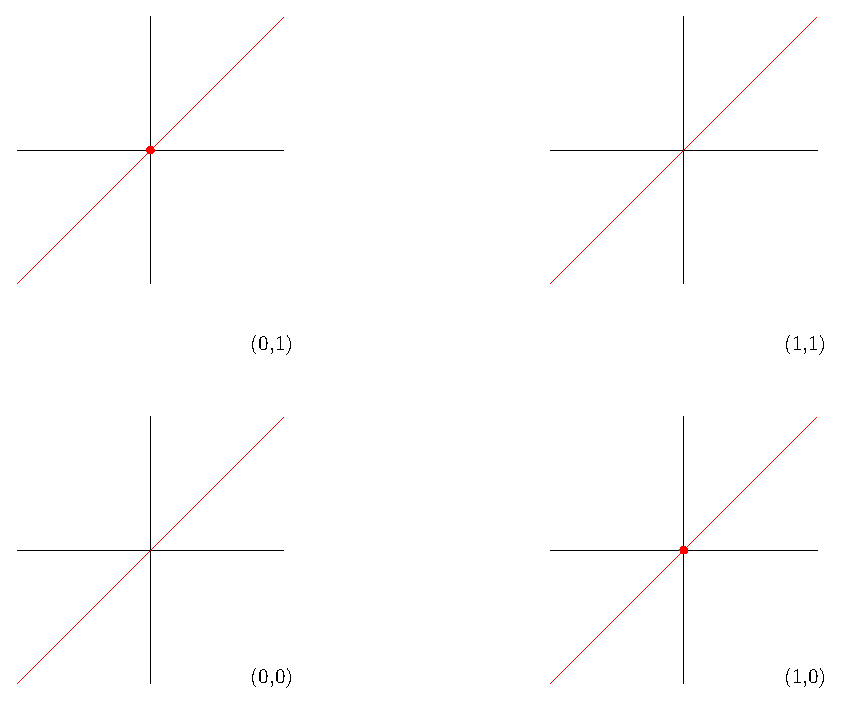
\includegraphics[width=0.8\textwidth]{graph.eps}
		\end{figure}
	\end{example}
	\begin{prop}
		Si $\quot{X}{\sim}$ est séparé, alors le graphe de la relation  $\sim$ est fermé.
	\end{prop}
	Pour arriver à ce résultat nous aurons besoin du Lemme suivant.
	\begin{lemma}
		Un espace est Hausdorff si et seulement si la diagonale $\Delta \defeq \{(x,x) \in X \times X\}$ est fermée.
	\end{lemma}
	\begin{proof}
		Soient $x \neq y \in X$ et  $x \in U, y \in V$ des voisinages distincts. Alors  $U\times V$ est un voisinage ouvert de  $(x,y) \in X\times Y$ munit de la topologie produit. On observe que  $U\cap V \neq \varnothing \iff U\times V \cap \Delta = \varnothing$. On peut séparer x et y par des ouverts si et seulement si $\Delta^c$ est ouvert.
	\end{proof}
	\begin{proof}[de la proposition]
		Si le quotient $\quot{X}{\sim}$est séparé, la diagonale $\Delta \subset (\quot{X}{\sim})^2$ est fermée par le Lemme précédent. On considère $q\times q : X \times X \longmapsto (\quot{X}{\sim}) \times (\quot{X}{\sim})$, continue et on identifie \[
			q^{-1}(\Delta) = \{(x,y) \;|\; [x] = [y]\} = \Gamma 
		\] qui est donc fermé.	
	\end{proof}
	Notons cependant que cette condition n'est pas suffisante. Le critère suivant donne une condition suffisante, bien que non nécessaire. On va utiliser $q^{-1}(q(A))$ pour  $A \subset X$ qu'on appelle des \emph{saturés} de A.

	\begin{prop}
		Si X est un espace séparé tel que $q^{-1}(q(x))$ est compact pour tout  $x\in X$ et $q^{-1}(q(F))$ est fermé dans X pour tout F fermé dans X, alors $\quot{X}{\sim} = q(X)$ est séparé
	\end{prop}
	\begin{proof}
		Prenons deux classes disjointes du quotient $[x] \neq [y]$. Puisque X est séparé on peut trouver deux ouverts disjoints de X U et V avec $q^{-1}(x) \in U$ et  $q^{-1}(y) \in V$ puisque $q^{-1}([x])$ et  $q^{-1}([y])$ sont compacts. En regardant les complémentaires fermés on a que \[
			U^c \subset q^{-1}(q(U^c)) \; \text{et} \; V^c \subset q^{-1}(q(V^c))
		.\] Soient donc \[
		U' \defeq X\setminus(q^{-1}(q(U^c))) \subset U \; \text{et} \; V' \defeq X\setminus(q^{-1}(q(V^c))) \subset V
	.\]  On va prouver que $q(U')$ et  $q(V')$ sont des voisinages ouverts et disjoints de $[x]$ et $[y]$ respectivement. 
	D'abord $[x] \in q(U')$ car  $x \neq q^{-1}(q(U^c))$ et de même  $[y] \in q(V')$. Pour montrer que $q(U')$ est ouvert, on montre que  $U' = q^{-1}(q(U'))$. La première inclusion est toujours vérifiée, montrons la seconde. Soit $u \in q^{-1}(q(U'))$, alors $q(u) \in q(U')$ et donc $q(u) \not\in q(U^c)$. Ainsi  $u \not\in q^{-1}(q(U^c))$, donc $u \in U'$ par construction de U', de même pour V'. \\
	Pour terminer la preuve, montrons que $q(U')$ et  $q(V')$ sont disjoints. Supposons par l'absurde que ce ne soit pas le cas, soit donc $[z] \in q(U')\cap q(V')$ il existe  $u' \in U'$ tel que  $[z] = q(u') \in q(V')$. Donc $u' \in q^{-1}(q(V')) = V'$ mais  $U'$ et  $V'$ sont disjoints, contradiction.
	Pour terminer la preuve notons 
	\end{proof}
	\begin{cor}
		Si $A \subset X$ est un sous espace compact et X séparé, alors $\quot{X}{A}$ est séparé.
	\end{cor}
	\begin{proof}
		Le critère précédent est vérifié puisque la saturation d'un point
		\begin{align*}
			q^{-1}(q(x)) = \begin{cases}
				A \; \text{si} \; x \in A \\
				\{x\} \; \text{sinon} 
			\end{cases}
		.\end{align*} Dans les deux cas ce sont des compacts.
		Si $F \subset X$ est fermé alors 
		\begin{align*}
			q^{-1}(q(F)) = \begin{cases}
				F \; \text{si} \; A\cap F = \varnothing \\
				F \cup A \; \text{sinon}
			\end{cases}
		.\end{align*}
	\end{proof}
	\begin{example} On montre à travers cet exemple que cette proposition n'est \emph{pas} nécessaire. On définit sur $\mathbf{R}^2$ la relation  \[
		\overrightarrow{x} \sim \overrightarrow{y} \iff \exists \overrightarrow{a} \in \mathbf{Z}^2 \;|\; \overrightarrow{x} + \overrightarrow{a} = \overrightarrow{y}
	.\] Alors $\quot{\mathbf{R}^2}{\sim}$ est compact et séparé mais $q^{-1}(q(\overrightarrow{0})) = \mathbf{Z}^2$ n'est pas compact.
	\end{example}

	\begin{definition}[Espace projectif réel]
		Soit $S^n \subset \mathbf{R}^{n+1}$ la sphère unité et $\sim$ la relation définie par $x \sim y \iff x = \pm y$ pour $x,y \in S^n$.
	\end{definition}
	\begin{prop}
		$\mathbf{R}P^n$ est compact et séparé.
	\end{prop}
	\begin{proof}
		$S^n$ est compact le quotient l'est aussi. De plus $q^{-1}(q(x)) = \{\pm x\}$ est compact et $q^{-1}(q(F)) = F \cup -F$ est fermé comme union de deux fermés et donc par la proposition précédente le quotient est séparé.
	\end{proof}
	On passe de $\mathbf{R}$ à  $\mathbf{C}$ et on remplace les nombre réels de valeur absolue 1 par  $S^1 \subset \mathbf{C}$ les nombres complexes de module 1.

	\begin{definition}[Espace projectif complexe]
		Soit $S^{2n+1} \subset \mathbf{C}^{n+1}$ la sphère unité et la relation $\sim$ définie par  $x \sim y  \iff x = a\cdot y$ pour un $a \in S^1$. Le quotient $\mathbf{C}P^n$ est l'espace projectif complexe de dimension  $n$.
	\end{definition}

	\section{Quotient par des actions de groupe}

	\begin{definition}[Groupe topologique]
		Un groupe topologique G est un ensemble m'unit d'une loi de groupe $\cdot$ ainsi que d'une topologie telle que la multiplication et l'inversion soient des applications continues. 
	\end{definition}

	\begin{example} On donne quelques exemples de base de groupes topologiques \\
		\begin{enumerate}
			\item Tout groupe munit de la topologie discrète est un groupe topologique, il est parfois noté $G^{\delta}$.
			\item $(\mathbf{R}^n,+)$ est un groupe topologique pour la topologie euclidienne.
			\item $(GL_n(\mathbf{R}),\cdot)$ est un groupe topologique muni de la topologie de sous espace de $M_n(\mathbf{R}) \cong \mathbf{R}^{n^2}$. La multiplication et inversion de matrice sont des applications continues. 
		\end{enumerate}	
	\end{example}

	\begin{lemma}
		Tout sous groupe d'un groupe topologique est encore un groupe topologique.
	\end{lemma}

	\begin{definition}
		Une action d'un groupe topologique G à droite sur un espace X est donnée par une application continue
		\begin{align*}
			X \times G &\longmapsto X \\
			(x,g) &\longmapsto x\cdot g
		\end{align*} satisfaisant 

		\begin{center}
			\begin{enumerate}
				\item $x \cdot 1_G = x$
				\item $x \cdot (gh) = (xg)\cdot h$
			\end{enumerate}
		\end{center}
	\end{definition}

	\begin{definition}[Espace des orbites]
		Soit X un espace sur lequel G agit. L'espace des orbites $\quot{X}{G}$ est le quotient de X par la relation $x \sim y \iff \exists g \in G \;|\; x = y \cdot g$.
	\end{definition}
\end{document}
